\section{La Circunferencia}
La circunferencia es una curva plana y cerrada que cuyos puntos son iguales de la distancia del centro
\begin{equation}
    (x)^{2} + (y )^{2} =r^{2}
\end{equation}

Para resolver estas ecuaciones es importante ubicar los 2 puntos que están localizadas a la misma distancia del centro
\begin{equation}
    (x - h)^{2} + (y - k)^{2} =r^{2}
\end{equation}

\begin {figure}[h!]
\centerline{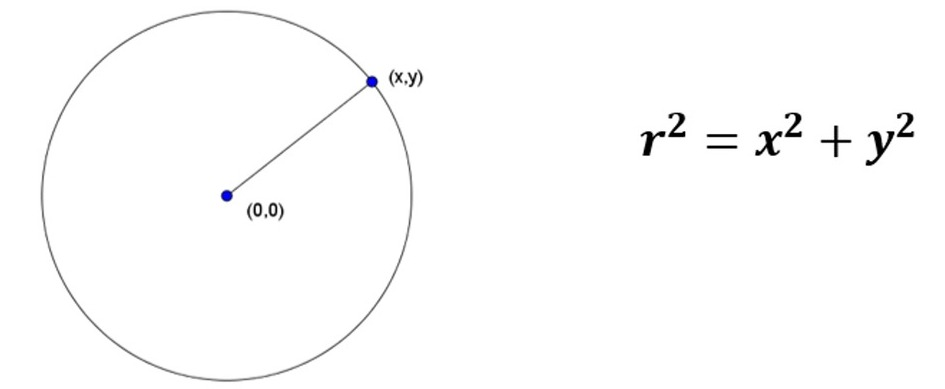
\includegraphics[width = 6cm]{Latex-imágenes/circunferencia2.jpeg}}
\caption{circunferencia}
\label{fig}
\end {figure}

\subsection{Círculo y Circunferencia}

Existe una gran confusión respecto a estas dos figuras, muchas veces empleadas como sinónimos, que guardan grandes similitudes, pero una diferencia bastante importante:
\begin{itemize}
\item la circunferencia es el lugar geométrico y el círculo una región del plano.
\end{itemize}

La circunferencia es una línea curva cuyos puntos distan igual respecto del centro. Por otro lado, el círculo es una región de puntos, un área, una superficie cuyos puntos se encuentran a una distancia no mayor al radio respecto del centro.

\begin {figure}[h!]
\centerline{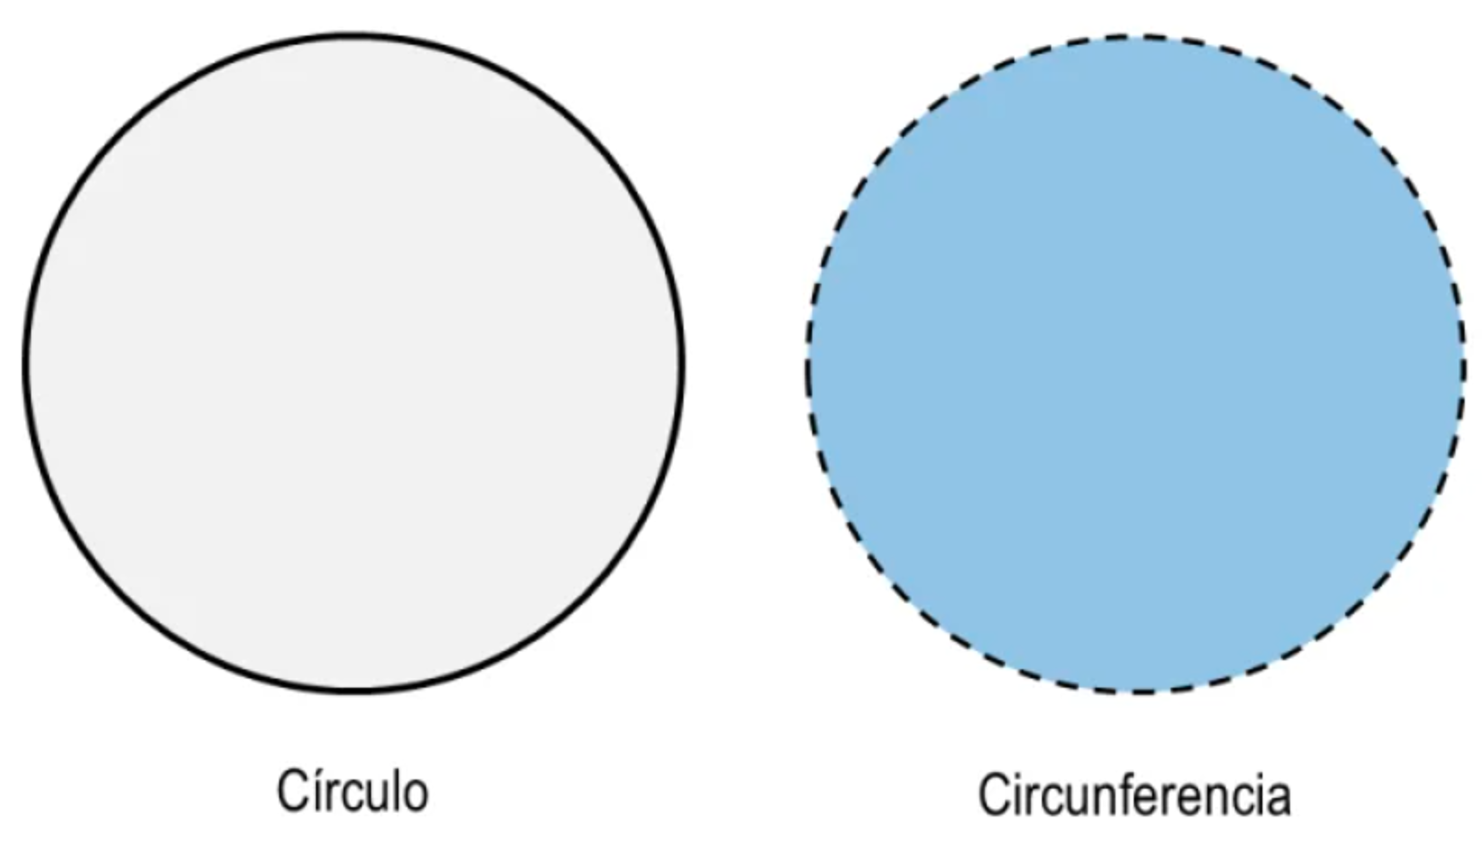
\includegraphics[width = 6cm]{Latex-imágenes/Circulo, Circunferencia.png}}
\caption{Circulo, Circunferencia}
\label{fig}
\end {figure}

\subsection{Descripción del problema}

Se solicita que una circunferencia con centro en el punto $C$ con coordenadas $(x_{1}, y_{1})$ y radio $r$, se evalué si un punto $T$ con coordenadas $(x_{2}, y_{2})$ esta dentro del área de la circunferencia.

\subsection{Definición de solución}

Primero tenemos que identificar las coordenadas de la circunferencia, que son las coordenadas del centro y así mismo también tenemos que conocer la distancia que hay del centro de la circunferencia hasta cualquier otro punto para así poder saber toda el área que abarca esta circunferencia.

\subsection{Diseño de Solución}
para poder determinar si un punto esta dentro de la circunferencia, primero tenemos que saber el centro de esta circunferencia $(x_{1}, y_{1})$ y a su vez también tenemos que saber la distancia de cualquier otro punto $(x_{2}, y_{2})$ el cual sera nuestro radio que nos ayudara a determinar el área que abarca nuestra circunferencia mediante la siguiente formula:
\begin{equation}
    A = \pi \cdot r^{2}
\end{equation}
Y posteriormente se le solicita al usuario las coordenadas $(x_{3}, y_{3})$ de su punto para determinar si este se encuentra dentro de la circunferencia.
\subsection{Desarrollo de Solución}

\begin{javaCode}
import java.util.Scanner;

public class Circunferencia {
    public static void main(String[] args) {
        Scanner scanner = new Scanner(System.in);
// 
        System.out.println("Ingrese las coordenadas del centro del circulo (x1, y1):");
        double x1 = scanner.nextDouble();
        double y1 = scanner.nextDouble();

        System.out.println("Ingrese las coordenadas de un punto en el circulo (x2, y2):");
        double x2 = scanner.nextDouble();
        double y2 = scanner.nextDouble();

        // Calcula el radio del circulo usando la fórmula de distancia entre dos puntos.
        double radio = Math.sqrt(Math.pow(x2 - x1, 2) + Math.pow(y2 - y1, 2));

        System.out.println("El área del círculo es: " + calcularArea(radio));

        System.out.println("Ingrese las coordenadas de un punto para verificar si esta dentro del círculo (x3, y3):");
        double x3 = scanner.nextDouble();
        double y3 = scanner.nextDouble();

        // Verifica si el punto (x3, y3) está dentro del círculo.
        boolean estaDentro = Math.pow(x3 - x1, 2) + Math.pow(y3 - y1, 2) <= Math.pow(radio, 2);

        if (estaDentro) {
            System.out.println("El punto está dentro del círculo.");
        } else {
            System.out.println("El punto está fuera del círculo.");
        }
    }

    public static double calcularArea(double radio) {
        return Math.PI * Math.pow(radio, 2);
    }
}
\end{javaCode}

\subsection{Depuración y pruebas}

\begin{table}[h]
\centering
\begin{tabular}{|c|c|c|c|c|}
  \hline
  Corrida & X1,Y1 & X2,Y2 & X3,Y3 & ¿El punto está dentro del círculo? \\
  \hline
  1 & 0,0 & 5,5 & 2,3 & SI \\
  \hline
  2 & 9,7 & 3,1 & 8,4 & SI \\
  \hline
  3 & 12,15 & 20,15 & 24,30 & NO \\
  \hline
\end{tabular}
\end{table}

\begin {figure}[h!]
\centerline{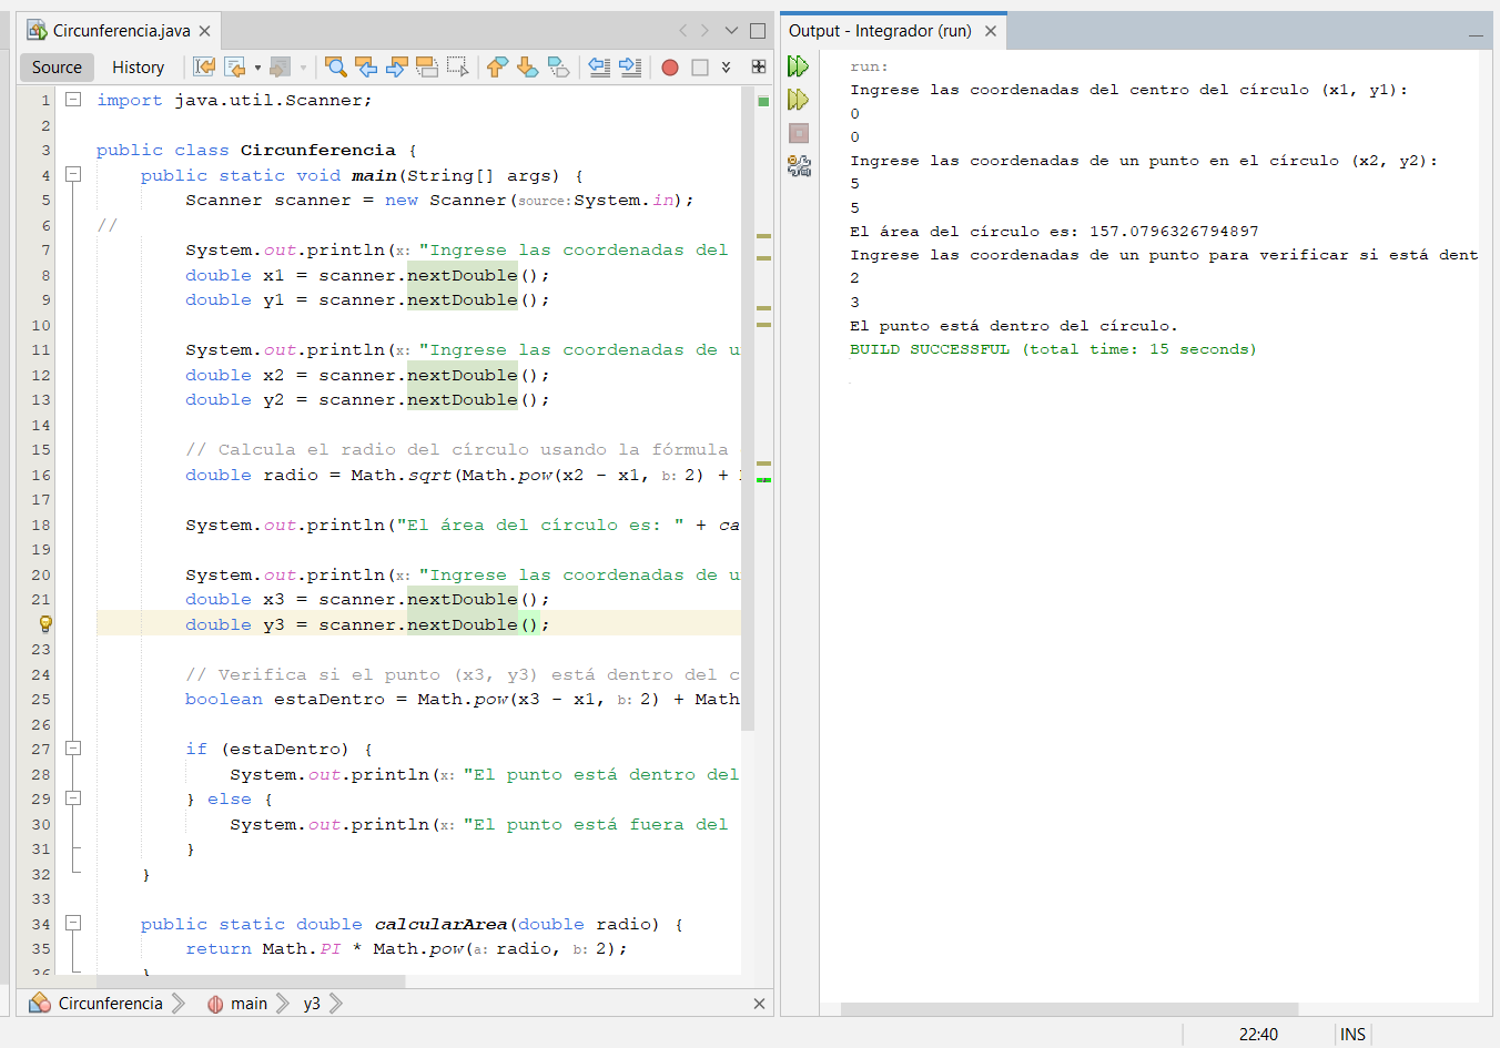
\includegraphics[width = 8cm]{Latex-imágenes/Corrida1_circunferencia.png}}
\caption{Corrida 1}
\label{fig}
\end {figure}

\begin {figure}[h!]
\centerline{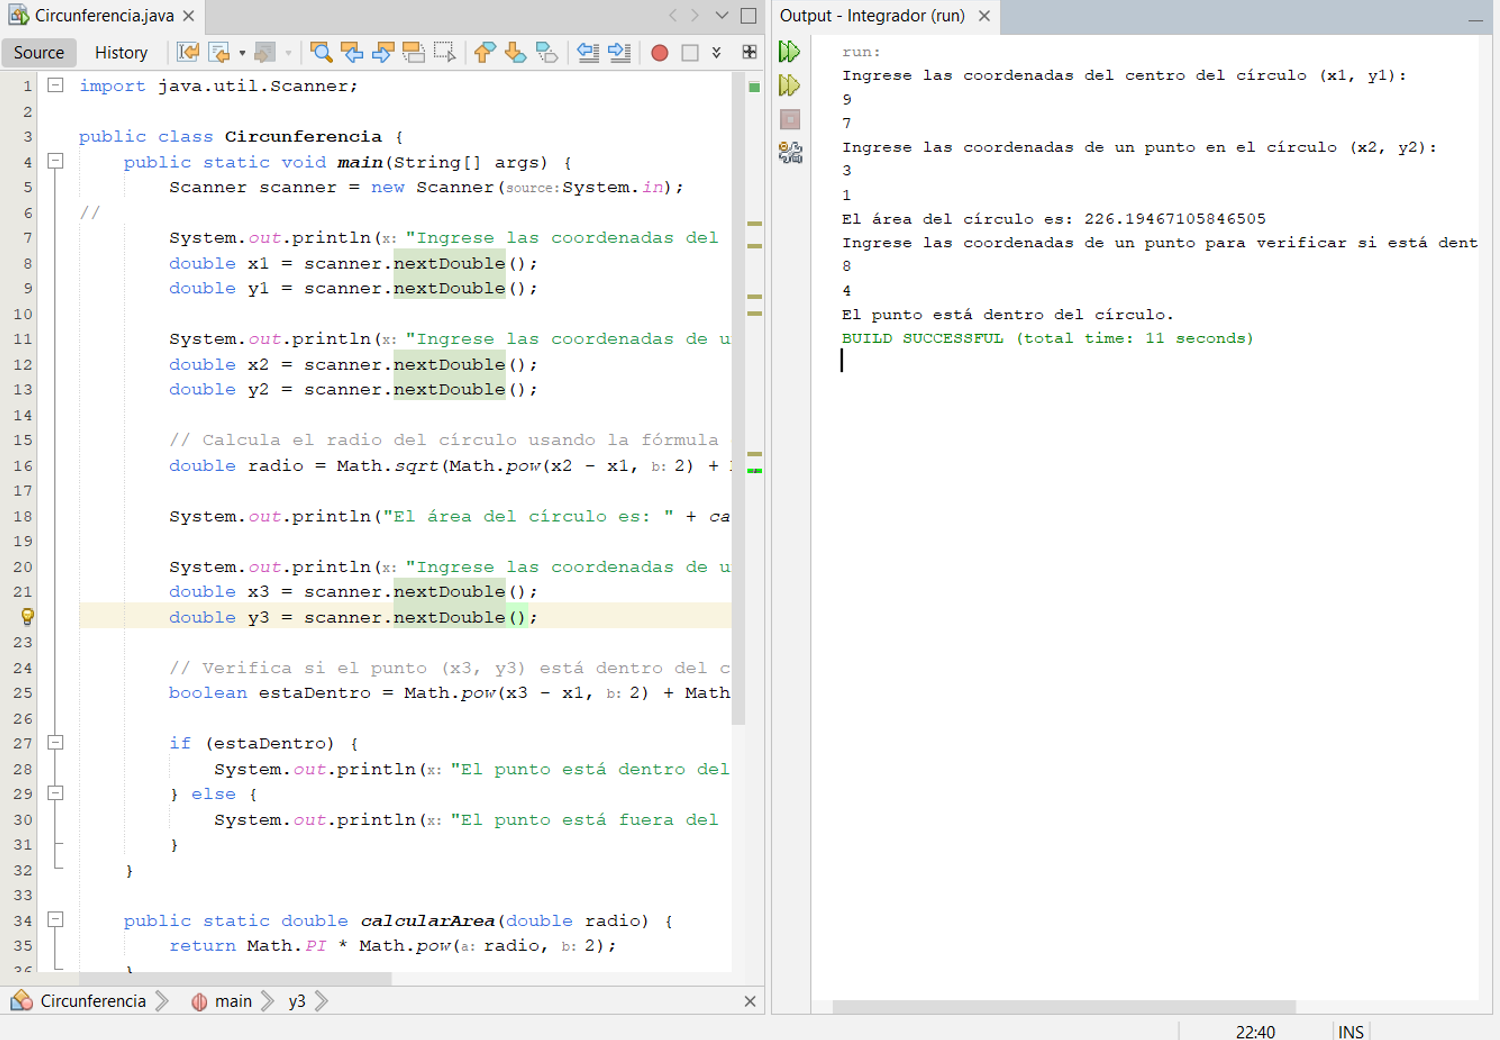
\includegraphics[width = 8cm]{Latex-imágenes/Corrida2_circunferencia.png}}
\caption{Corrida 2}
\label{fig}
\end {figure}

\begin {figure}[h!]
\centerline{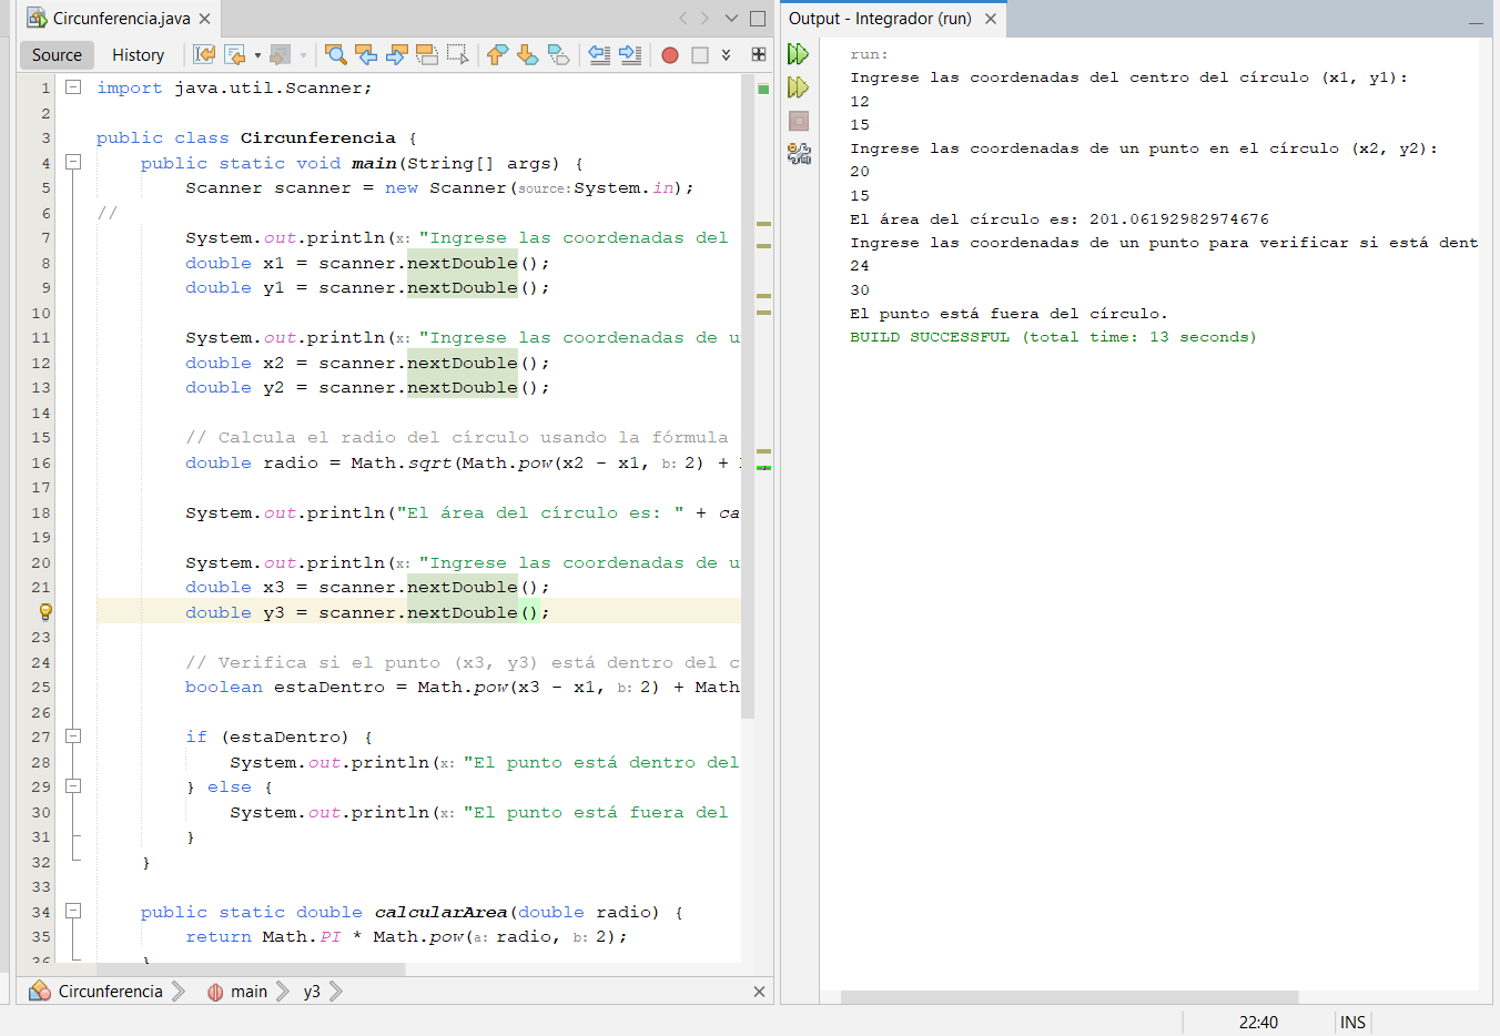
\includegraphics[width = 8cm]{Latex-imágenes/Corrida3_circunferencia.png}}
\caption{Corrida 3}
\label{fig}
\end {figure}